\documentclass[border=10pt]{standalone}
\usepackage{karnaugh-map}
\usepackage{tikz}

\begin{document}
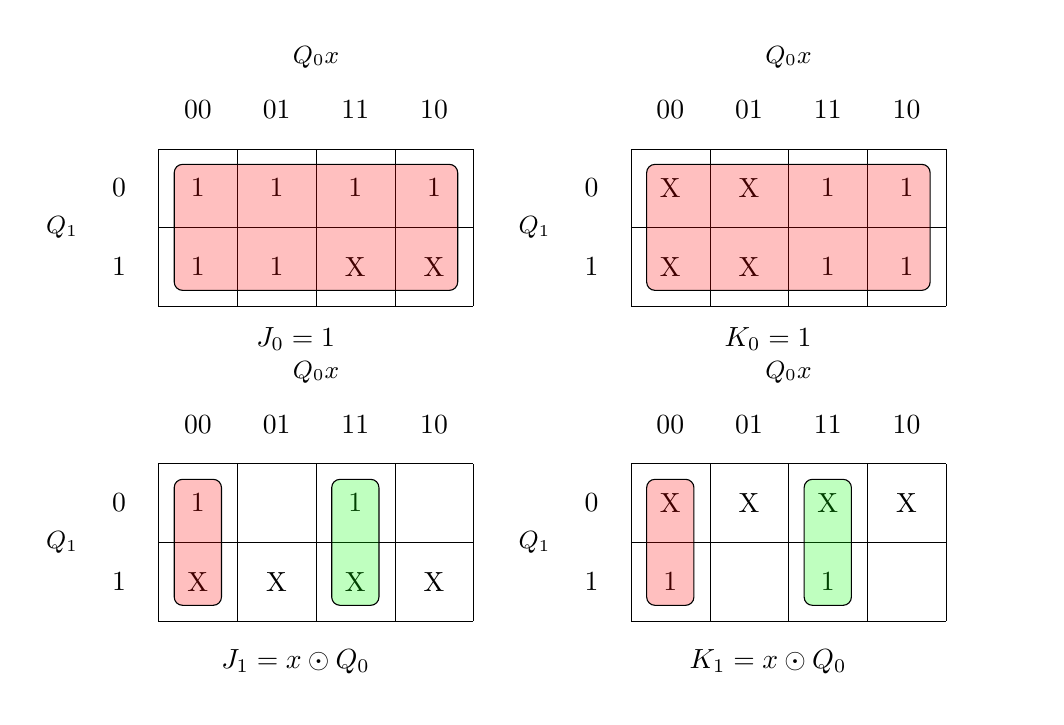
\begin{tikzpicture}
    % J0
    \node at (0, 4) {
        \begin{karnaugh-map}[4][2][1][$Q_0x$][$Q_1$]
            \minterms{0,1,2,3,4,5}
            \autoterms[X]
            \implicant{0}{6} % Covers everything
        \end{karnaugh-map}
    };
    \node at (0, 2.3) {$J_0 = 1$};

    % K0
    \node at (6, 4) {
        \begin{karnaugh-map}[4][2][1][$Q_0x$][$Q_1$]
            \minterms{2,3,6,7}
            \autoterms[X]
            % Wait, recall K0 table:
            % 000: X, 001: X. Q0=0 cases are X.
            % 010 (Q0=1, x=0): 1
            % 011 (Q0=1, x=1): 1
            % 100: X, 101: X.
            % 110: 1, 111: 1.
            % Indices: 0, 1, 4, 5 are X.
            % Indices: 2, 3, 6, 7 are 1.
            % Group 2,3,6,7.
            \implicant{0}{6}
        \end{karnaugh-map}
    };
    \node at (6, 2.3) {$K_0 = 1$};

    % J1
    \node at (0, 0) {
        \begin{karnaugh-map}[4][2][1][$Q_0x$][$Q_1$]
            % J1 values:
            % 000 (0): 1
            % 001 (1): 0
            % 010 (2): 0
            % 011 (3): 1
            % Q1=1 (4,5,6,7): X
            \minterms{0,3}
            \terms{4,5,6,7}{X}
            % Grouping: x XOR Q0
            % Group 0 with 4 (corner to corner not great visually, but logic-wise)
            % Wait, X conditions allow simplifying.
            % 0 (000), 4 (100 is X) -> Group 0,4 = x'Q0'
            % 3 (011), 7 (111 is X) -> Group 3,7 = xQ0
            \implicant{0}{4}
            \implicant{3}{7}
        \end{karnaugh-map}
    };
    \node at (0, -1.8) {$J_1 = x \odot Q_0$};

    % K1
    \node at (6, 0) {
        \begin{karnaugh-map}[4][2][1][$Q_0x$][$Q_1$]
            % K1 values:
            % Q1=0 (0,1,2,3): X
            % 100 (4): 1
            % 101 (5): 0
            % 110 (6): 0
            % 111 (7): 1
            \minterms{4,7}
            \terms{0,1,2,3}{X}
            % Group 4 (100) with 0(X) -> x'Q0'
            % Group 7 (111) with 3(X) -> xQ0
            \implicant{0}{4}
            \implicant{3}{7}
        \end{karnaugh-map}
    };
    \node at (6, -1.8) {$K_1 = x \odot Q_0$};

\end{tikzpicture}
\end{document}
